\chapter{Biodiversiteit op elke schaal}\label{ch:g10:biodiversity-scales}

Leg een vierkant van één meter touw op een gazon en tel wat erbinnen
groeit: gras natuurlijk, maar ook klaver, madeliefjes, een paardenbloem,
weegbree, mos, en, als je met een loep kijkt, een tiental insecten en
een slak. Verleg het vierkant naar het asfalt van de parkeerplaats:
niets, of één onkruid in een scheur. Verleg het naar een oud
graslandperceel dat nooit is geploegd: veertig plantensoorten, en
insecten in overvloed. Het woord voor wat het vierkant meet is
\emph{\omterm{def:g10:biodiversity-scales:biodiversity}{biodiversiteit}}, en dit hoofdstuk gaat over hoe je haar meet, op
welke schalen zij bestaat, en waarom zij niet vaststaat en niet
vanzelfsprekend is.

\section{Drie schalen van diversiteit}

\begin{definition}[Biodiversiteit]\label{def:g10:biodiversity-scales:biodiversity}
\emph{Biodiversiteit}\index{biodiversiteit} is de verscheidenheid van
levende wezens, beschouwd op drie schalen:
\begin{itemize}
  \item de verscheidenheid van \emph{ecosystemen}\index{ecosysteem} ---
        van de levensgemeenschappen en de omgevingen die zij innemen
        (een vijver, een beukenbos, een koraalrif, een grasland), elk
        met een eigen verzameling \omterm{def:g10:biodiversity-scales:species}{soorten};
  \item de verscheidenheid van \omterm{def:g10:biodiversity-scales:species}{soorten} binnen een
        ecosysteem of op aarde --- het aantal \omterm{def:g10:biodiversity-scales:species}{soorten} en hun onderlinge
        talrijkheid;
  \item de \emph{genetische diversiteit}\index{genetische diversiteit}
        binnen een \omterm{def:g10:biodiversity-scales:species}{soort} --- het aantal \omterm{def:g10:universal-dna:gene}{allelen} van haar \omterm{def:g10:universal-dna:gene}{genen} en de
        manier waarop die over haar individuen en populaties zijn
        verdeeld.
\end{itemize}
\end{definition}

\begin{omfigure}
\begin{tikzpicture}[font=\small, >=Stealth]
  \node[draw, rounded corners, thick, fill=omMeth!8, minimum width=11.4cm, minimum height=4.9cm] (eco) at (0,0) {};
  \node[anchor=north west, font=\small\bfseries] at (eco.north west) {\ ecosystemen: vijver, bos, rif, grasland\dots};
  \node[draw, rounded corners, thick, fill=omDef!10, minimum width=8.2cm, minimum height=3.2cm] (sp) at (0.6,-0.45) {};
  \node[anchor=north west, font=\small\bfseries] at (sp.north west) {\ soorten van één ecosysteem};
  \foreach \x/\t in {-2.6/kikker, -1.1/salamander, 0.4/libel, 1.9/riet, 3.4/waterlelie}
    \node[draw, fill=white, rounded corners=2pt, font=\scriptsize] at (\x,-0.3) {\t};
  \node[draw, rounded corners, thick, fill=omProp!12, minimum width=6.4cm, minimum height=1.2cm] (al) at (1.0,-1.35) {};
  \node[anchor=west, font=\scriptsize\bfseries] at (al.west) {\ allelen van één soort:};
  \foreach \x/\t in {1.6/a, 2.2/b, 2.8/c, 3.4/d, 4.0/e}
    \node[draw, circle, fill=white, inner sep=1.5pt, font=\scriptsize] at (\x,-1.35) {\t};
\end{tikzpicture}

{\small De drie in elkaar geschoven schalen van \omterm{def:g10:biodiversity-scales:biodiversity}{biodiversiteit}. Een
vijver verliezen betekent een gemeenschap van \omterm{def:g10:biodiversity-scales:species}{soorten} verliezen; een
\omterm{def:g10:biodiversity-scales:species}{soort} verliezen betekent al haar \omterm{def:g10:universal-dna:gene}{allelen} verliezen; \omterm{def:g10:universal-dna:gene}{allelen} verliezen
verarmt een \omterm{def:g10:biodiversity-scales:species}{soort} die nog bestaat.}
\end{omfigure}

\begin{definition}[Soort]\label{def:g10:biodiversity-scales:species}
Een \emph{soort}\index{soort} is een groep levende wezens die op elkaar lijken, zich
onderling kunnen voortplanten en vruchtbare nakomelingen krijgen; twee
populaties die zich niet met elkaar kunnen voortplanten, of waarvan de
kruisingen onvruchtbaar zijn, vormen verschillende soorten. In de
praktijk --- bij fossielen, bij bacteriën, bij organismen die nooit zijn
waargenomen bij de voortplanting --- worden soorten herkend aan hun
gedeelde kenmerken, en
\cref{ch:g12:selection-drift-speciation} zal laten zien dat de grens
niet altijd scherp is.
\end{definition}

\begin{example}[Paard, ezel, muildier]\label{ex:g10:biodiversity-scales:mule}
Een paard en een ezel lijken op elkaar en kunnen zich onderling
voortplanten: hun nakomeling is het muildier. Maar het muildier is
onvruchtbaar, dus zijn paard en ezel twee \omterm{def:g10:biodiversity-scales:species}{soorten}. Een poedel en een
Ierse wolfshond lijken in niets op elkaar, paren moeiteloos en geven
vruchtbare pups: één \omterm{def:g10:biodiversity-scales:species}{soort}, de hond --- die zich ook met de wolf, haar
voorouder, kan voortplanten.
\end{example}

\section{De verscheidenheid van soorten}

\begin{proposition}[Soorten tellen]\label{prop:g10:biodiversity-scales:count}
Er zijn ongeveer twee miljoen \omterm{def:g10:biodiversity-scales:species}{soorten} beschreven en benoemd. De meeste
zijn insecten (meer dan een miljoen), gevolgd door planten (zo'n
300\,000), schimmels, spinachtigen en weekdieren; de gewervelden, de
groep die wij het best kennen, tellen ongeveer 70\,000 \omterm{def:g10:biodiversity-scales:species}{soorten}, waarvan
6\,400 zoogdieren. Het aantal nog niet beschreven \omterm{def:g10:biodiversity-scales:species}{soorten} wordt, uit het
tempo waarin nieuwe worden gevonden, op nog enkele miljoenen geschat ---
misschien acht tot tien miljoen eukaryote \omterm{def:g10:biodiversity-scales:species}{soorten} in totaal, plus een
enorme, grotendeels ongetelde verscheidenheid aan bacteriën.
\end{proposition}
\admitted

\begin{omfigure}
\begin{tikzpicture}
\begin{axis}[
  xbar, bar width=7pt,
  width=0.8\linewidth, height=6.4cm,
  axis x line=bottom, axis y line=left,
  xmin=0, xmax=1200,
  xlabel={beschreven soorten (duizendtallen)},
  xlabel style={font=\small, at={(axis description cs:0.5,-0.1)}, anchor=north},
  symbolic y coords={zoogdieren, vogels, vissen, weekdieren, spinachtigen, schimmels, planten, insecten},
  ytick=data, tick label style={font=\small},
  enlarge y limits=0.1,
  nodes near coords, nodes near coords style={font=\scriptsize, anchor=west},
  xtick={0,200,400,600,800,1000,1200},
]
\addplot[fill=omDef!55, draw=omDef] coordinates
  {(6.4,zoogdieren) (11,vogels) (34,vissen) (85,weekdieren) (100,spinachtigen)
   (150,schimmels) (300,planten) (1000,insecten)};
\end{axis}
\end{tikzpicture}

{\small Beschreven \omterm{def:g10:biodiversity-scales:species}{soorten} in enkele grote groepen, in duizendtallen. De
groepen die wij het best kennen zijn de kleinste; alleen al de insecten
overtreffen alle gewervelden vijftien tegen één.}
\end{omfigure}

\begin{method}[De diversiteit van een terrein meten]\label{met:g10:biodiversity-scales:sampling}
Een terrein wordt nooit volledig geteld; er wordt \emph{bemonsterd}.
\begin{enumerate}
  \item Kies een monstereenheid die bij de organismen past: een kwadraat
        van \qty{1}{m^2} voor graslandplanten, een sleepnetslag voor
        insecten, een zeef met grond voor regenwormen, een lengte
        transect voor vogels.
  \item Leg de eenheden willekeurig of op vaste afstanden, en neem er
        genoeg dat één eenheid erbij het totaal nauwelijks nog
        verandert.
  \item Bepaal en tel in elke eenheid. Twee getallen beschrijven het
        monster: de \emph{soortenrijkdom}, het aantal gevonden \omterm{def:g10:biodiversity-scales:species}{soorten},
        en de \emph{relatieve talrijkheid} van elke \omterm{def:g10:biodiversity-scales:species}{soort} --- een
        terrein waar één \omterm{def:g10:biodiversity-scales:species}{soort} 95\% van de individuen levert, is minder
        divers dan een terrein waar tien \omterm{def:g10:biodiversity-scales:species}{soorten} hen gelijk verdelen,
        ook bij gelijke rijkdom.
  \item Vergelijk terreinen alleen met dezelfde methode en dezelfde
        inspanning, in hetzelfde seizoen.
\end{enumerate}
\end{method}

\begin{example}[Twee gazons]\label{ex:g10:biodiversity-scales:lawns}
Tien kwadraten op een gemaaid schoolgazon: 6 plantensoorten, waarvan
gras 90\% bedekt. Tien kwadraten op een ongemaaide berm ernaast: 23
\omterm{def:g10:biodiversity-scales:species}{soorten}, geen enkele boven 30\%. De berm is rijker en gelijkmatiger; het
verschil is niet de bodem of het klimaat, die gelijk zijn, maar het
maaien, dat elke plant verwijdert die niet vlak boven de grond kan
bloeien.
\end{example}

\begin{omfigure}
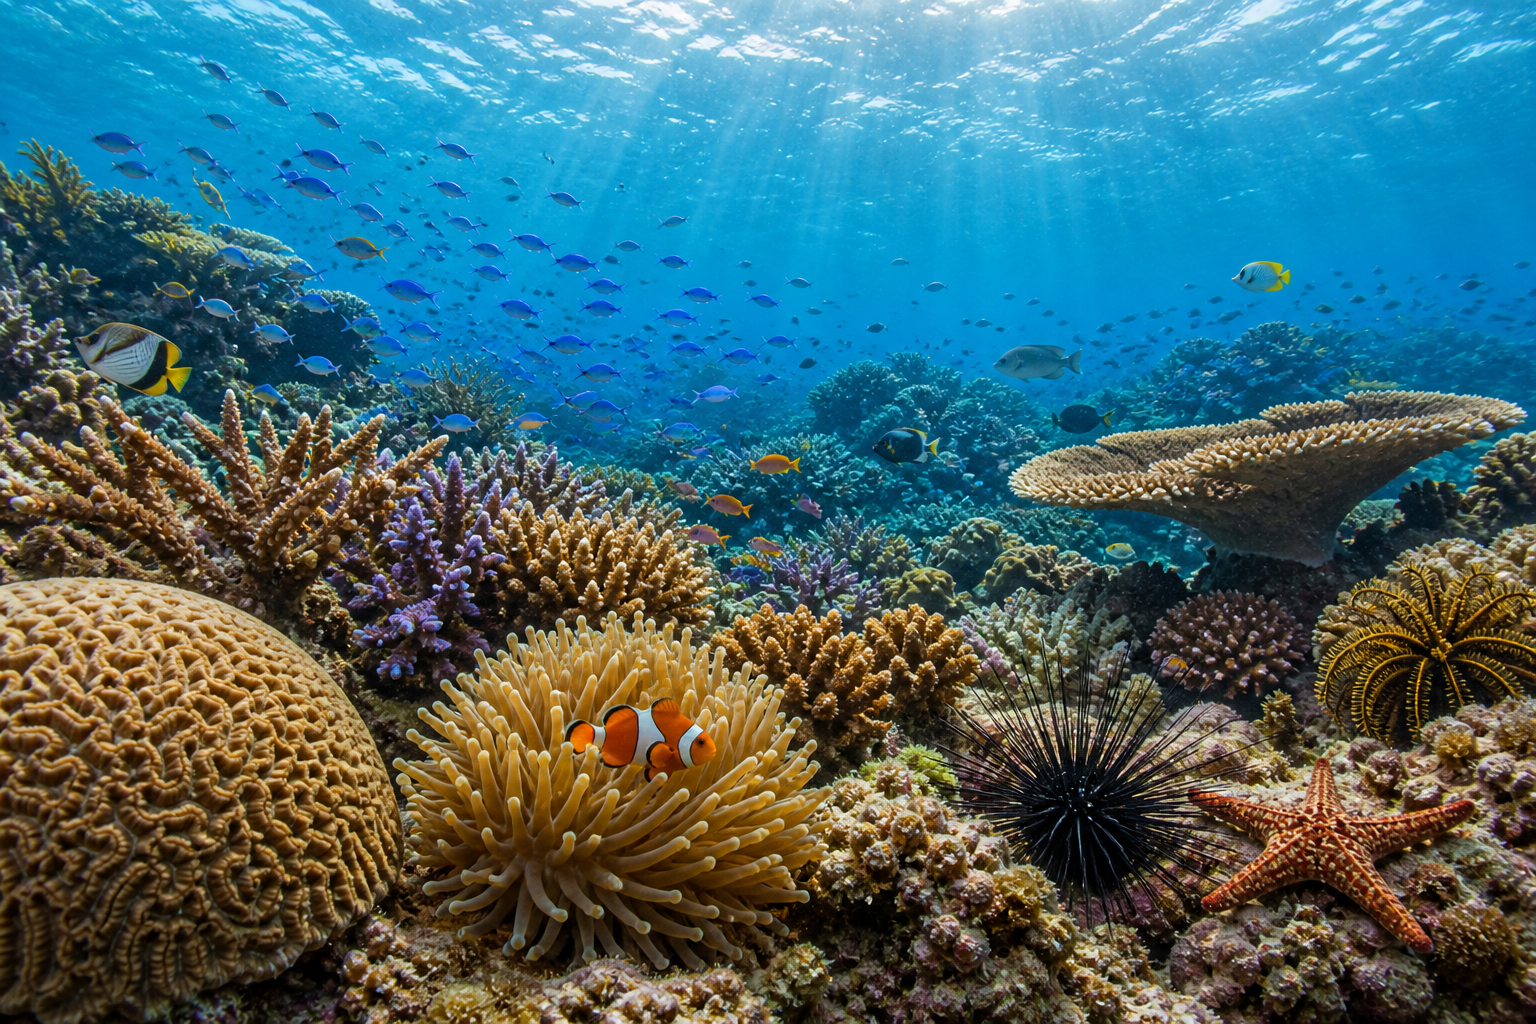
\includegraphics[width=0.66\linewidth]{images/book2/ai/g10-biodiv-coral-reef.png}

{\small Een koraalrif: op enkele vierkante meters koralen, vissen,
weekdieren, stekelhuidigen en anemonen van tientallen \omterm{def:g10:biodiversity-scales:species}{soorten}. Riffen
herbergen een kwart van alle zeesoorten op een tiende procent van de
zeebodem.}
\end{omfigure}

\section{Genetische diversiteit binnen een soort}

\begin{proposition}[Individuen van een soort zijn niet gelijk]\label{prop:g10:biodiversity-scales:genetic}
Binnen een \omterm{def:g10:biodiversity-scales:species}{soort} bestaan de meeste \omterm{def:g10:universal-dna:gene}{genen} in verscheidene \omterm{def:g10:universal-dna:gene}{allelen}, en de
individuen dragen daarvan verschillende combinaties. De
\emph{frequentie} van een \omterm{def:g10:universal-dna:gene}{allel} in een populatie --- het deel van alle
kopieën van het \omterm{def:g10:universal-dna:gene}{gen} dat dit \omterm{def:g10:universal-dna:gene}{allel} is --- verschilt van populatie tot
populatie. \omterm{def:g10:biodiversity-scales:biodiversity}{Genetische diversiteit} is wat een \omterm{def:g10:biodiversity-scales:species}{soort} in staat stelt te
reageren op een veranderende omgeving: een populatie waarin elk individu
gelijk is, heeft niets om uit te kiezen.
\end{proposition}
\admitted

\begin{example}[Allelen van de bloedgroepen over de wereld]\label{ex:g10:biodiversity-scales:abo}
Het \omterm{def:g10:universal-dna:gene}{gen} van de ABO-bloedgroepen heeft drie veelvoorkomende \omterm{def:g10:universal-dna:gene}{allelen}: A, B
en O. In West-Europa zijn hun frequenties ongeveer 0.27, 0.07 en 0.66;
in Oost-Azië ongeveer 0.20, 0.20 en 0.60; in sommige inheemse populaties
van Zuid-Amerika haalt het \omterm{def:g10:universal-dna:gene}{O-allel} alleen al 0.98. Dezelfde \omterm{def:g10:biodiversity-scales:species}{soort},
hetzelfde \omterm{def:g10:universal-dna:gene}{gen}, een andere verdeling van de \omterm{def:g10:universal-dna:gene}{allelen}: de \omterm{def:g10:biodiversity-scales:biodiversity}{genetische
diversiteit} van de mens is werkelijk, en zij is over de populaties
verspreid in plaats van ze op te splitsen --- het grootste deel van de
diversiteit van de \omterm{def:g10:biodiversity-scales:species}{soort} is binnen elke afzonderlijke populatie terug
te vinden.
\end{example}

\begin{omfigure}
\begin{tikzpicture}
\begin{axis}[
  ybar, bar width=9pt,
  width=0.8\linewidth, height=5.2cm,
  axis x line=bottom, axis y line=left,
  ymin=0, ymax=1.1, ylabel={allelfrequentie}, ylabel style={font=\small},
  symbolic x coords={West-Europa, Oost-Azië, Andes},
  xtick=data, tick label style={font=\small},
  enlarge x limits=0.25,
  legend style={at={(0.5,-0.2)}, anchor=north, legend columns=3,
                font=\small, draw=none},
  ytick={0,0.2,0.4,0.6,0.8,1.0},
]
\addplot[fill=omThm!50, draw=omThm] coordinates {(West-Europa,0.27) (Oost-Azië,0.20) (Andes,0.01)};
\addplot[fill=omProp!50, draw=omProp] coordinates {(West-Europa,0.07) (Oost-Azië,0.20) (Andes,0.01)};
\addplot[fill=omDef!50, draw=omDef] coordinates {(West-Europa,0.66) (Oost-Azië,0.60) (Andes,0.98)};
\legend{allel A, allel B, allel O}
\end{axis}
\end{tikzpicture}

{\small Bij benadering de frequenties van de drie \omterm{def:g10:universal-dna:gene}{ABO-allelen} in drie
menselijke populaties. De drie frequenties van een populatie tellen op
tot 1.}
\end{omfigure}

\begin{example}[Een soort met vrijwel geen]\label{ex:g10:biodiversity-scales:cheetah}
Jachtluipaarden lijken genetisch zo sterk op elkaar dat huidtransplantaten
tussen niet-verwante dieren worden aangenomen alsof het tweelingen
betreft: de \omterm{def:g10:biodiversity-scales:species}{soort} is zo'n tienduizend jaar geleden door een flessenhals
van heel weinig individuen gegaan en heeft haar \omterm{def:g10:universal-dna:gene}{allelen} nooit
teruggekregen. Welke nieuwe ziekte of welk nieuw klimaat ook komt, elk
jachtluipaard treedt die met dezelfde uitrusting tegemoet; de \omterm{def:g10:biodiversity-scales:species}{soort}
overleeft, maar zonder iets in reserve.
\end{example}

\section{Biodiversiteit verandert: vroeger, nu}

\begin{proposition}[Biodiversiteit is een toestand, geen constante]\label{prop:g10:biodiversity-scales:changes}
De verzameling \omterm{def:g10:biodiversity-scales:species}{soorten} die op een gegeven moment leeft, is een stadium
in een geschiedenis. Het fossielenarchief toont \omterm{def:g10:biodiversity-scales:species}{soorten} die verschijnen,
gemiddeld enkele miljoenen jaren voortbestaan en verdwijnen; de totale
verscheidenheid van het leven is over de laatste 540 miljoen jaar
toegenomen, onderbroken door vijf
\emph{massa-uitstervingen}\index{massa-uitsterving} waarbij meer dan
drie kwart van de \omterm{def:g10:biodiversity-scales:species}{soorten} binnen een geologisch korte tijd verdween. De
jongste, 66 miljoen jaar geleden, maakte een einde aan de niet-vogelige
dinosauriërs en opende de weg voor de opsplitsing van de zoogdieren.
\end{proposition}
\begin{proof}[Bewijsmateriaal]
Tellingen van fossiele families in gedateerde gesteentelagen, voor het
hele mariene archief samengebracht, leveren de kromme van de volgende
figuur: een stijging van enkele honderden tot bijna duizend families,
met scherpe dalen 445, 370, 252, 201 en 66 miljoen jaar geleden. De
gebeurtenis van 252 miljoen jaar geleden, de grootste, verwijderde
ongeveer 95\% van de mariene \omterm{def:g10:biodiversity-scales:species}{soorten}; de lagen er vlak boven zijn bijna
leeg van fossielen, en nieuwe groepen vullen ze pas in de miljoenen
jaren daarna.
\end{proof}

\begin{omfigure}
\begin{tikzpicture}
\begin{axis}[
  width=0.9\linewidth, height=5.6cm,
  axis x line=bottom, axis y line=left,
  x dir=reverse, xmin=0, xmax=560, ymin=0, ymax=1100,
  xlabel={miljoenen jaren geleden}, ylabel={mariene diersoortenfamilies},
  xlabel style={font=\small, at={(axis description cs:0.5,-0.12)}, anchor=north},
  ylabel style={font=\small},
  tick label style={font=\small}, xtick={500,400,300,200,100,0},
  ytick={0,200,400,600,800,1000},
  clip=false,
]
\addplot[thick, omDef] coordinates
  {(540,120) (520,300) (490,420) (460,500) (447,510) (440,400)
   (420,470) (380,530) (368,540) (360,450) (330,480) (300,520)
   (260,540) (252,560) (248,300) (230,380) (210,440) (202,450)
   (196,380) (150,520) (100,650) (70,760) (66,780) (62,650)
   (40,760) (20,880) (0,1000)};
\draw[thick, omThm, ->] (axis cs:445,760) -- (axis cs:445,600);
\node[font=\scriptsize, omThm, anchor=south] at (axis cs:445,770) {1};
\draw[thick, omThm, ->] (axis cs:370,790) -- (axis cs:370,630);
\node[font=\scriptsize, omThm, anchor=south] at (axis cs:370,800) {2};
\draw[thick, omThm, ->] (axis cs:252,820) -- (axis cs:252,660);
\node[font=\scriptsize, omThm, anchor=south] at (axis cs:252,830) {3};
\draw[thick, omThm, ->] (axis cs:201,700) -- (axis cs:201,540);
\node[font=\scriptsize, omThm, anchor=south] at (axis cs:201,710) {4};
\draw[thick, omThm, ->] (axis cs:66,1030) -- (axis cs:66,870);
\node[font=\scriptsize, omThm, anchor=south] at (axis cs:66,1040) {5};
\end{axis}
\end{tikzpicture}

{\small Aantal families van zeedieren door de tijd, uit het
fossielenarchief, met de vijf \omterm{prop:g10:biodiversity-scales:changes}{massa-uitstervingen} aangegeven (1: einde
van het Ordovicium; 2: laat-Devoon; 3: einde van het Perm, de grootste;
4: einde van het Trias; 5: einde van het Krijt). De diversiteit stijgt in
het geheel, en op elke instorting volgt een traag herstel.}
\end{omfigure}

\begin{proposition}[De verandering van nu]\label{prop:g10:biodiversity-scales:present}
\omterm{def:g10:biodiversity-scales:species}{Soorten} verdwijnen op dit ogenblik met een tempo dat wordt geschat op
honderd tot duizend keer het gemiddelde van het fossielenarchief, door
de vernietiging van \omterm{def:g10:biodiversity-scales:biodiversity}{ecosystemen} (bosontginning, drooglegging van
moerassen, verstedelijking), door overexploitatie, door ingevoerde
\omterm{def:g10:biodiversity-scales:species}{soorten}, door vervuiling en door klimaatverandering --- alle van
menselijke oorsprong. De helft van de tropische bossen van 1950 is
verdwenen; een derde van de amfibieënsoorten wordt bedreigd; de
\omterm{def:g10:biodiversity-scales:biodiversity}{genetische diversiteit} van gewassen en vee is teruggebracht tot enkele
rassen. \omterm{def:g10:biodiversity-scales:biodiversity}{Biodiversiteit} is een hulpbron --- voedsel, geneesmiddelen,
bestuiving, bodem, de stabiliteit van \omterm{def:g10:biodiversity-scales:biodiversity}{ecosystemen} --- en haar verlies is
op menselijke tijdschaal niet omkeerbaar.
\end{proposition}
\admitted

\begin{example}[Een verlies terugdraaien]\label{ex:g10:biodiversity-scales:reversing}
Waar houtwallen die in de jaren zestig zijn verwijderd opnieuw zijn
aangeplant, keert de rijkdom aan vogels en insecten binnen een tiental
jaar terug; waar in 1995 wolven in een nationaal park zijn
teruggebracht, hielden de herten waarop zij jagen op de wilgen langs de
rivier kaal te vreten, groeiden de wilgen terug, kwamen de bevers terug,
en met hen de vogels en vissen die van beverpoelen afhankelijk zijn. Een
\omterm{def:g10:biodiversity-scales:biodiversity}{ecosysteem} beschermen of herstellen herstelt de diversiteit op alle drie
de schalen tegelijk; een \omterm{def:g10:biodiversity-scales:species}{soort} die in een dierentuin in leven wordt
gehouden, behoudt er slechts één van.
\end{example}

\section{Oefeningen}

\begin{exercise}[$\star$]\label{exo:g10:biodiversity-scales:1}
Noem de drie schalen van \omterm{def:g10:biodiversity-scales:biodiversity}{biodiversiteit} en geef van elk een voorbeeld.
\end{exercise}

\begin{exercise}[$\star$]\label{exo:g10:biodiversity-scales:2}
Definieer een \omterm{def:g10:biodiversity-scales:species}{soort}. Zijn de leeuw en de tijger --- die in gevangenschap
onvruchtbare kruisingen kunnen geven --- één \omterm{def:g10:biodiversity-scales:species}{soort} of twee?
\end{exercise}

\begin{exercise}[$\star$]\label{exo:g10:biodiversity-scales:3}
Hoeveel keer meer insectensoorten dan zoogdiersoorten zijn er volgens de
soortengrafiek beschreven?
\end{exercise}

\begin{exercise}[$\star$]\label{exo:g10:biodiversity-scales:4}
Wat is een allelfrequentie? Wat is in een populatie waarin het \omterm{def:g10:universal-dna:gene}{O-allel}
frequentie 0.66 heeft en het \omterm{def:g10:universal-dna:gene}{A-allel} 0.27, de frequentie van B?
\end{exercise}

\begin{exercise}[$\star$]\label{exo:g10:biodiversity-scales:5}
Hoeveel \omterm{prop:g10:biodiversity-scales:changes}{massa-uitstervingen} toont het fossielenarchief, en welke was de
grootste?
\end{exercise}

\begin{exercise}[$\star\star$]\label{exo:g10:biodiversity-scales:6}
Twee graslanden hebben elk 12 plantensoorten. In het eerste levert één
\omterm{def:g10:biodiversity-scales:species}{soort} 80\% van de planten; in het tweede komt geen \omterm{def:g10:biodiversity-scales:species}{soort} boven 15\%.
Welk van beide is diverser, en welk van de twee getallen uit
\cref{met:g10:biodiversity-scales:sampling} onderscheidt hen?
\end{exercise}

\begin{exercise}[$\star\star$]\label{exo:g10:biodiversity-scales:7}
Een leerling telt insecten in 3 sleepnetslagen en vindt 8 \omterm{def:g10:biodiversity-scales:species}{soorten}; een
klasgenoot doet 30 slagen in hetzelfde veld en vindt er 21. Heeft het
veld voor de klasgenoot meer \omterm{def:g10:biodiversity-scales:species}{soorten}? Leg uit wat het verschil laat zien
over bemonsteren.
\end{exercise}

\begin{exercise}[$\star\star$]\label{exo:g10:biodiversity-scales:8}
Leg uit waarom een \omterm{def:g10:biodiversity-scales:species}{soort} die tot enkele tientallen individuen is
teruggebracht, in gevaar kan blijven ook nadat haar aantallen weer tot
in de duizenden zijn gegroeid.
\end{exercise}

\begin{exercise}[$\star\star$]\label{exo:g10:biodiversity-scales:9}
Lees in de figuur van de fossiele families het aantal families vlak vóór
en vlak na de uitsterving van 252 miljoen jaar geleden af, en bereken het
verloren deel. Waarom is het verloren deel van de \emph{\omterm{def:g10:biodiversity-scales:species}{soorten}} groter
dan dat van de families?
\end{exercise}

\begin{exercise}[$\star\star$]\label{exo:g10:biodiversity-scales:10}
Leg met \cref{ex:g10:biodiversity-scales:abo} uit in welke zin twee
buren in dezelfde stad genetisch waarschijnlijk ongeveer evenveel van
elkaar verschillen als twee mensen van verschillende werelddelen.
\end{exercise}

\begin{exercise}[$\star\star$]\label{exo:g10:biodiversity-scales:11}
Een vijver wordt gedempt om er een parkeerplaats te bouwen. Noem één
verlies op elk van de drie schalen van \omterm{def:g10:biodiversity-scales:biodiversity}{biodiversiteit}.
\end{exercise}

\begin{exercise}[$\star\star\star$]\label{exo:g10:biodiversity-scales:12}
De gemiddelde \omterm{def:g10:biodiversity-scales:species}{soort} uit het fossielenarchief bestaat enkele miljoenen
jaren; schat met twee miljoen bekende \omterm{def:g10:biodiversity-scales:species}{soorten} het "achtergrondaantal"
uitstervingen per jaar. Als het huidige tempo duizend keer hoger ligt,
hoeveel \omterm{def:g10:biodiversity-scales:species}{soorten} zouden er dan per jaar verdwijnen, en hoeveel per eeuw?
\end{exercise}

\begin{exercise}[$\star\star\star$]\label{exo:g10:biodiversity-scales:13}
Na de uitsterving van 66 miljoen jaar geleden splitsten de zoogdieren
zich binnen zo'n 20 miljoen jaar van enkele kleine vormen op in
walvissen, vleermuizen, olifanten en primaten. Leg uit hoe een ramp voor
de \omterm{def:g10:biodiversity-scales:biodiversity}{biodiversiteit} ook een oorzaak van nieuwe \omterm{def:g10:biodiversity-scales:biodiversity}{biodiversiteit} kan zijn.
\end{exercise}

\begin{exercise}[$\star\star\star$]\label{exo:g10:biodiversity-scales:14}
De moderne tarwe stamt af van een handvol rassen; haar wilde verwanten
groeien in de bergen van het Nabije Oosten. Leg met het begrip
\omterm{def:g10:biodiversity-scales:biodiversity}{genetische diversiteit} uit waarom zaadbanken de wilde verwanten bewaren,
ook al leveren die niets bruikbaars op.
\end{exercise}

\begin{exercise}[$\star\star\star$]\label{exo:g10:biodiversity-scales:15}
"Uitsterven is natuurlijk, dus is er geen reden om je over het huidige
uitsterven zorgen te maken." Bespreek dit in een alinea, met het tempo
van uitsterven, de hersteltijd en de hulpbronnen die \omterm{def:g10:biodiversity-scales:biodiversity}{biodiversiteit}
levert.
\end{exercise}

\section{Probleem: Het rendement van de houtwal}

\begin{problem}[{Weekendprobleem --- een veldopname op twee boerderijen,
één met en één zonder houtwallen: soorten geteld, talrijkheden
vergeleken, de allelen van een slak gevolgd, en het getal dat een
houtwal waard is}]
\label{pb:g10:biodiversity-scales:1}
Twee naburige boerderijen verbouwen dezelfde tarwe op dezelfde grond.
Boerderij A behield haar houtwallen; boerderij B verwijderde ze in 1970.
Een klas bemonstert beide in juni met dezelfde methode: 20 kwadraten van
\qty{1}{m^2} langs de akkerranden voor planten, 20 sleepnetslagen voor
insecten, en 10 minuten luisteren op 5 punten voor vogels.

\medskip
\noindent\textbf{Deel I --- Planten.}
Uitkomsten, boerderij A: 31 plantensoorten in de 20 kwadraten;
boerderij B: 9. Op boerderij B levert één grassoort 84\% van de getelde
planten; op boerderij A levert de gewoonste \omterm{def:g10:biodiversity-scales:species}{soort} 22\%.
\begin{enumerate}
  \item Geef de soortenrijkdom van de randen van elke boerderij en de
        verhouding daartussen.
  \item Welke plantengemeenschap is gelijkmatiger? Leg uit wat
        "gelijkmatig" toevoegt aan "rijk".
  \item Op boerderij A bedroeg het aantal gevonden \omterm{def:g10:biodiversity-scales:species}{soorten} na 5, 10, 15
        en 20 kwadraten 18, 25, 29 en 31. Is de bemonstering toereikend?
        Verantwoord dat.
  \item Dezelfde reeks op boerderij B was 6, 8, 9, 9. Vergelijk de twee
        reeksen en zeg welke vorm een "volledige" bemonsteringskromme
        aanneemt.
  \item Waarom moeten beide boerderijen in dezelfde maand worden
        bemonsterd?
\end{enumerate}

\medskip
\noindent\textbf{Deel II --- Insecten en vogels.}
Insecten: boerderij A 46 \omterm{def:g10:biodiversity-scales:species}{soorten}, boerderij B 14. Vogels: boerderij A 17
\omterm{def:g10:biodiversity-scales:species}{soorten}, boerderij B 5; op boerderij B behoorde 60\% van de gehoorde
vogels tot één \omterm{def:g10:biodiversity-scales:species}{soort}.
\begin{enumerate}[resume]
  \item Bereken de verhouding van de insectenrijkdom en van de
        vogelrijkdom tussen de boerderijen. Vertellen de drie groepen
        (planten, insecten, vogels) hetzelfde verhaal?
  \item Stel een keten van oorzaken voor die het verwijderen van de
        houtwallen verbindt met de daling van de insectendiversiteit, en
        vervolgens met die van de vogels.
  \item De tarweopbrengst per hectare is op beide boerderijen gelijk.
        Betekent dat dat de houtwallen geen invloed op het gewas hebben?
        Noem één dienst die een houtwal kan bewijzen en die het
        opbrengstcijfer niet laat zien.
  \item Noem één \omterm{def:g10:biodiversity-scales:species}{soort} die de klas alleen op boerderij A zou verwachten,
        en leg uit waarom.
  \item Welke schaal van \omterm{def:g10:biodiversity-scales:biodiversity}{biodiversiteit} is op boerderij B het duidelijkst
        verkleind: \omterm{def:g10:biodiversity-scales:biodiversity}{ecosystemen}, \omterm{def:g10:biodiversity-scales:species}{soorten} of \omterm{def:g10:universal-dna:gene}{genen}? Verantwoord dat.
\end{enumerate}

\medskip
\noindent\textbf{Deel III --- De \omterm{def:g10:universal-dna:gene}{allelen} van een slak.}
De gewone tuinslak draagt een \omterm{def:g10:universal-dna:gene}{gen} met twee veelvoorkomende \omterm{def:g10:universal-dna:gene}{allelen} voor
de schelpkleur, geel (g) en bruin (b). In de houtwallen van boerderij A
zijn 400 slakken bemonsterd: 100 hebben twee \omterm{def:g10:universal-dna:gene}{g-allelen}, 200 hebben één g
en één b, 100 hebben twee b. Op de ene overgebleven wal van boerderij B,
100 slakken: 4 met twee g, 32 met één van elk, 64 met twee b.
\begin{enumerate}[resume]
  \item Tel de kopieën van g en van b in elk monster (elke slak draagt
        twee kopieën). Leid daaruit de frequentie van g op elke
        boerderij af.
  \item Welke populatie is voor dit \omterm{def:g10:universal-dna:gene}{gen} genetisch diverser? Vergelijk het
        aandeel slakken dat beide \omterm{def:g10:universal-dna:gene}{allelen} draagt.
  \item Lijsters jagen op slakken op het zicht; op de kale wal van
        boerderij B zijn bruine schelpen beter verborgen. Stel voor hoe
        de frequenties van boerderij B tot stand zijn gekomen.
  \item Als een vochtige, beschaduwde houtwal gele schelpen bevoordeelde,
        wat zou je dan voor de slakken van boerderij B voorspellen als
        de houtwallen werden herplant en er verder niets veranderde?
  \item De slakken van boerderij B tellen enkele honderden, die van
        boerderij A tienduizenden. Welke populatie loopt meer kans een
        \omterm{def:g10:universal-dna:gene}{allel} geheel toevallig kwijt te raken? Waarom?
\end{enumerate}

\medskip
\noindent\textbf{Deel IV --- Het rendement.}
\begin{enumerate}[resume]
  \item Bereken over de drie groepen heen de totale soortenrijkdom van
        elke boerderij, en vervolgens het totaal van A gedeeld door dat
        van B.
  \item De houtwallen van boerderij A beslaan 3\% van haar oppervlakte.
        Zeg in één zin welk deel van het land welk deel van de \omterm{def:g10:biodiversity-scales:species}{soorten}
        herbergt.
  \item Houtwallen die in 1995 op boerderij B zijn herplant, werden in
        2010 opnieuw opgenomen: 24 plantensoorten, 35 insectensoorten,
        12 vogelsoorten. Welk deel van de rijkdom van boerderij A had
        elke groep teruggekregen?
  \item Welke van de drie schalen van \omterm{def:g10:biodiversity-scales:biodiversity}{biodiversiteit} herstelt na
        herplanting het traagst, en waarom?
  \item Geef het resultaat: de factor waarmee houtwallen de soortenrijkdom
        van een boerderij vermenigvuldigden, en de ene schaal van
        \omterm{def:g10:biodiversity-scales:biodiversity}{biodiversiteit} die een herplante houtwal niet uit zichzelf kan
        terugbrengen.
\end{enumerate}
\end{problem}
